\documentclass[conference]{IEEEtran}

\usepackage{cite}
\usepackage{amsmath,amssymb,amsfonts}
\usepackage{graphicx}
\usepackage{textcomp}
\usepackage{xcolor}
\usepackage{booktabs}
\usepackage{array}
\usepackage{url}
\renewcommand{\ttdefault}{cmtt}
\makeatletter
\newcommand{\tabinput}[1]{\@@input #1 }
\makeatother

\graphicspath{{../figures/}}
\renewcommand{\figurename}{Gambar}
\renewcommand{\tablename}{TABEL}
\renewcommand{\abstractname}{Abstrak}
\renewcommand{\IEEEkeywordsname}{Kata kunci}
\renewcommand{\refname}{Referensi}

\begin{document}

\title{Pengaruh Jumlah Data serta Augmentasi Rotasi dan \emph{Brightness} terhadap Ketahanan MobileNetV2 Beku pada CIFAR-10}

\author{\IEEEauthorblockN{Carlo Angkisan}
\IEEEauthorblockA{\textit{Program Studi Teknik Informatika} \\
\textit{Sekolah Teknik Elektro dan Informatika}\\
\textit{Institut Teknologi Bandung}\\
Bandung, Indonesia \\
13523091@std.stei.itb.ac.id}
}

\maketitle

\begin{abstract}
Penelitian ini mengukur seberapa jauh fitur MobileNetV2 hasil \emph{pretraining} ImageNet tetap berguna ketika data latih sangat sedikit dan citra uji mengalami gangguan visual. \emph{Backbone} dibekukan dan fitur diekstrak satu kali, lalu hanya \emph{linear head} yang dilatih pada \emph{subset} CIFAR-10 berukuran 250 atau 1000 citra, masing-masing dengan dan tanpa augmentasi rotasi dan \emph{brightness}. Setiap kondisi diulang dengan tiga \emph{seed} dan dievaluasi pada \emph{test} bersih serta enam gangguan sintetis. Menambah data dari 250 ke 1000 citra menaikkan macro-F1 \emph{test} bersih sebesar 4,02 pp tanpa augmentasi dan 6,78 pp dengan augmentasi, dengan arah yang sama di ketiga \emph{seed}. Augmentasi menurunkan macro-F1 \emph{test} bersih pada 250 citra ($-$2,09 pp), tetapi sedikit menaikkannya pada 1000 citra (+0,67 pp). Manfaat terbesar augmentasi terlihat pada rotasi. Penurunan macro-F1 akibat rotasi 20° berkurang kira-kira setengahnya, baik pada 250 maupun 1000 citra. Manfaat ini tidak berpindah ke \emph{blur}, dan augmentasi \emph{brightness} tidak memperbaiki ketahanan terhadap citra gelap secara konsisten. Hasil ini menunjukkan bahwa augmentasi untuk \emph{backbone} beku sebaiknya dipilih sesuai jenis gangguan yang diperkirakan muncul, dan manfaatnya tidak bisa diasumsikan ketika datanya sangat sedikit.
\end{abstract}

\begin{IEEEkeywords}
augmentasi data, CIFAR-10, data terbatas, ketahanan model, MobileNetV2, \emph{transfer learning}
\end{IEEEkeywords}

\section{Pendahuluan}

CNN yang dilatih pada ImageNet sering dipakai ulang sebagai ekstraktor fitur untuk tugas lain. Cara paling murah adalah membekukan seluruh \emph{backbone} dan hanya melatih \emph{classifier} linear di atas fiturnya \cite{donahue2014decaf}. Pendekatan ini cocok untuk kondisi dengan data berlabel sedikit dan komputasi terbatas. Dalam praktik, ada dua pertanyaan yang langsung muncul. Pertama, berapa banyak data yang sebenarnya dibutuhkan. Kedua, apakah model masih bisa diandalkan ketika citra yang masuk lebih gelap, buram, atau miring dibanding data latih. Studi ketahanan seperti Hendrycks dan Dietterich \cite{hendrycks2019benchmarking} umumnya menguji model yang dilatih penuh dengan data besar, sehingga perilaku \emph{backbone} beku dengan data sangat sedikit belum banyak dibahas.

Penelitian ini menjawab kedua pertanyaan itu dengan eksperimen terkontrol memakai \emph{backbone} MobileNetV2 \cite{sandler2018mobilenetv2}, resolusi \emph{input} 128$\times$128, serta augmentasi \emph{training} berupa rotasi dan \emph{brightness}. Empat kondisi \emph{training} (E1--E4) membandingkan 250 dan 1000 citra latih, masing-masing dengan dan tanpa augmentasi. Setiap kondisi dijalankan dengan tiga \emph{seed} dan diuji pada tujuh kondisi \emph{test}. Seluruh konfigurasi, termasuk \emph{hyperparameter}, ditetapkan sejak awal dan tidak diubah setelah melihat hasil \emph{test}. Fokusnya adalah perbandingan yang adil dan dapat diaudit, bukan mencari skor tertinggi.

Hasil utamanya ada tiga. Penambahan data menaikkan macro-F1 secara konsisten di hampir semua kondisi. Augmentasi rotasi dan \emph{brightness} sangat membantu terhadap rotasi tetapi tidak terhadap gangguan lain. Selain itu, \emph{pipeline} yang dibangun menghasilkan metrik dan prediksi kelas yang sama persis ketika dijalankan di mesin yang berbeda.

\section{Kajian Terkait}\label{sec:related}

\subsection{Fitur \emph{Pretrained} sebagai Ekstraktor Tetap}

Donahue dkk.\ \cite{donahue2014decaf} menunjukkan bahwa aktivasi CNN yang dilatih pada ImageNet \cite{deng2009imagenet} dapat dipakai untuk tugas pengenalan lain cukup dengan \emph{classifier} sederhana. Razavian dkk.\ \cite{razavian2014cnn} memperkuat temuan ini: fitur \emph{off-the-shelf} ditambah SVM linear sudah menjadi \emph{baseline} yang sulit dikalahkan di banyak \emph{dataset}. Yosinski dkk.\ \cite{yosinski2014transferable} menjelaskan bahwa fitur lapisan akhir makin spesifik terhadap tugas asal, sehingga daya transfernya turun ketika tugas target makin berbeda. Kornblith dkk.\ \cite{kornblith2019better} menemukan bahwa akurasi ImageNet berkorelasi kuat dengan kinerja transfer, termasuk pada skenario fitur tetap dengan regresi logistik. Penelitian ini memakai skenario fitur tetap yang sama, tetapi dengan data latih yang jauh lebih sedikit, yaitu 25 dan 100 citra per kelas.

MobileNetV2 \cite{sandler2018mobilenetv2} memakai blok \emph{inverted residual} dengan \emph{linear bottleneck} dan menghasilkan vektor 1280 dimensi setelah \emph{global average pooling}. Arsitektur ini dirancang untuk perangkat dengan sumber daya terbatas. CIFAR-10 \cite{krizhevsky2009cifar} berisi citra 32$\times$32 piksel, jauh lebih kecil dari resolusi ImageNet, sehingga citra perlu diperbesar sebelum masuk ke \emph{backbone}.

\subsection{Ketahanan terhadap Gangguan Visual}

Hendrycks dan Dietterich \cite{hendrycks2019benchmarking} menyusun CIFAR-10-C dan ImageNet-C untuk mengukur penurunan kinerja model terhadap gangguan umum seperti \emph{blur}, \emph{noise}, dan perubahan kecerahan. Dodge dan Karam \cite{dodge2016quality} melaporkan bahwa \emph{blur} dan \emph{noise} menurunkan akurasi CNN cukup besar, sedangkan perubahan kontras dan kompresi JPEG berdampak lebih kecil. Untuk transformasi geometris, Azulay dan Weiss \cite{azulay2019small} menunjukkan bahwa pergeseran atau perubahan skala kecil saja dapat mengubah keluaran CNN. Engstrom dkk.\ \cite{engstrom2019spatial} menemukan bahwa rotasi dan translasi kecil yang dipilih secara terburuk dapat menurunkan akurasi secara drastis, dan augmentasi data biasa hanya sedikit membantu terhadap kasus terburuk tersebut. Studi-studi tersebut umumnya menguji model yang seluruh lapisannya dilatih. Penelitian ini justru membekukan \emph{backbone}, sehingga yang diukur adalah seberapa jauh \emph{linear head} saja dapat menyesuaikan diri terhadap gangguan.

\subsection{Augmentasi dan Variasi Eksperimen}

Survei Shorten dan Khoshgoftaar \cite{shorten2019survey} merangkum augmentasi geometris dan fotometris yang umum dipakai. Manfaatnya bergantung pada apakah transformasi tersebut mempertahankan label dan seberapa mirip dengan variasi yang muncul saat pengujian. Bouthillier dkk.\ \cite{bouthillier2021variance} menunjukkan bahwa pemilihan sampel data, inisialisasi parameter, dan pilihan \emph{hyperparameter} sama-sama berpengaruh nyata pada hasil \emph{benchmark}, sehingga perbandingan sebaiknya dilaporkan atas beberapa percobaan. Mengikuti saran tersebut, setiap kondisi di penelitian ini dijalankan dengan tiga \emph{seed} dan konsistensi arah perbedaannya diperiksa. Augmentasi yang diuji juga sengaja sejenis dengan sebagian gangguan \emph{test}, sehingga dapat dilihat apakah manfaatnya terbatas pada gangguan yang sejenis.

\section{Metode}\label{sec:method}

Setiap citra $x$ dilewatkan ke \emph{backbone} beku $\phi$ untuk menghasilkan fitur $\phi(x) \in \mathbb{R}^{1280}$. Yang dilatih hanya \emph{linear head} $z(x) = W\phi(x) + b$ dengan $W \in \mathbb{R}^{10 \times 1280}$. Karena \emph{backbone} tidak berubah, fitur cukup diekstrak satu kali lalu disimpan sebagai \emph{cache}, dan seluruh \emph{training} serta evaluasi memakai \emph{cache} tersebut. Empat kondisi \emph{training} (E1--E4) dibandingkan, masing-masing dengan tiga \emph{seed}, lalu diuji pada tujuh kondisi \emph{test}.

\subsection{Data dan \emph{Split}}

Eksperimen memakai sepuluh kelas CIFAR-10. Untuk setiap kelas $c$, indeks \emph{split train} resmi diurutkan lalu diacak dengan generator acak ber-\emph{seed} $2026 + c$. Seratus indeks pertama menjadi \emph{train} penuh, 50 berikutnya menjadi \emph{validation}, dan 25 indeks pertama dari \emph{train} penuh menjadi \emph{train} terbatas. \emph{Test} diambil dari \emph{split test} resmi dengan cara yang sama memakai \emph{seed} $3026 + c$. Jumlah sampelnya ditunjukkan pada Tabel~\ref{tab:split}. \emph{Split} yang sama dipakai untuk semua \emph{training seed}. \emph{Train} dan \emph{validation} tidak beririsan, dan \emph{train} terbatas merupakan bagian dari \emph{train} penuh.

\begin{table}[t]
\caption{Jumlah sampel per \emph{split}. Setiap kelas mendapat jumlah yang sama.}
\label{tab:split}
\centering
\begin{tabular}{lrr}
\toprule
Bagian & Per kelas & Total \\
\midrule
\tabinput{tables/jumlah_sampel.tex}
\bottomrule
\end{tabular}
\end{table}

\subsection{\emph{Preprocessing} dan Ekstraksi Fitur}

Setiap citra dikonversi ke RGB, di-\emph{resize} langsung dari 32$\times$32 ke 128$\times$128 dengan interpolasi \emph{bilinear} dan \emph{antialiasing}, diubah ke rentang 0--1, lalu dinormalisasi dengan \emph{mean} dan \emph{standard deviation} ImageNet. Tidak ada \emph{crop}, \emph{flip}, atau operasi lain. Resolusi 128 dipakai sebagai kondisi eksperimen, bukan mengikuti resolusi standar ImageNet.

\emph{Backbone} MobileNetV2 memakai bobot ImageNet \texttt{IMAGENET1K\_V1} dari torchvision. \emph{Classifier} bawaannya dibuang dan semua parameternya dibekukan. Ekstraksi dijalankan dalam mode evaluasi tanpa perhitungan gradien, sehingga BatchNorm memakai statistik berjalan hasil \emph{pretraining} \cite{ioffe2015batchnorm} dan fitur satu citra tidak bergantung pada isi \emph{batch}-nya. Fitur $\phi(x)$ diambil dari keluaran blok konvolusi terakhir lalu diringkas dengan \emph{global average pooling}. Bobot \emph{backbone} dibandingkan sebelum dan sesudah ekstraksi untuk memastikan tidak ada yang berubah.

Fitur diekstrak satu kali untuk sepuluh \emph{cache}, yaitu \emph{train} bersih, \emph{train} augmentasi, \emph{validation} bersih, dan tujuh kondisi \emph{test}, dengan total 9500 citra.

\subsection{Augmentasi \emph{Training}}

Setiap citra \emph{train} penuh mendapat tepat satu versi augmentasi tetap. Dari generator acak ber-\emph{seed} 2026 ditambah indeks asli citra, diambil sudut rotasi $\theta \sim U(-10^\circ, 10^\circ)$ lalu faktor \emph{brightness} $\beta \sim U(0{,}7;\ 1{,}3)$. Rotasi (interpolasi \emph{bilinear}, area kosong diisi 0) diterapkan lebih dulu, kemudian \emph{brightness}. Keduanya diterapkan setelah \emph{resize} dan sebelum normalisasi (Gambar~\ref{fig:aug}), dan selalu diterapkan bersama pada setiap citra, bukan dipilih salah satu. Parameter tiap sampel disimpan bersama \emph{cache}.

\begin{figure}[t]
\centering
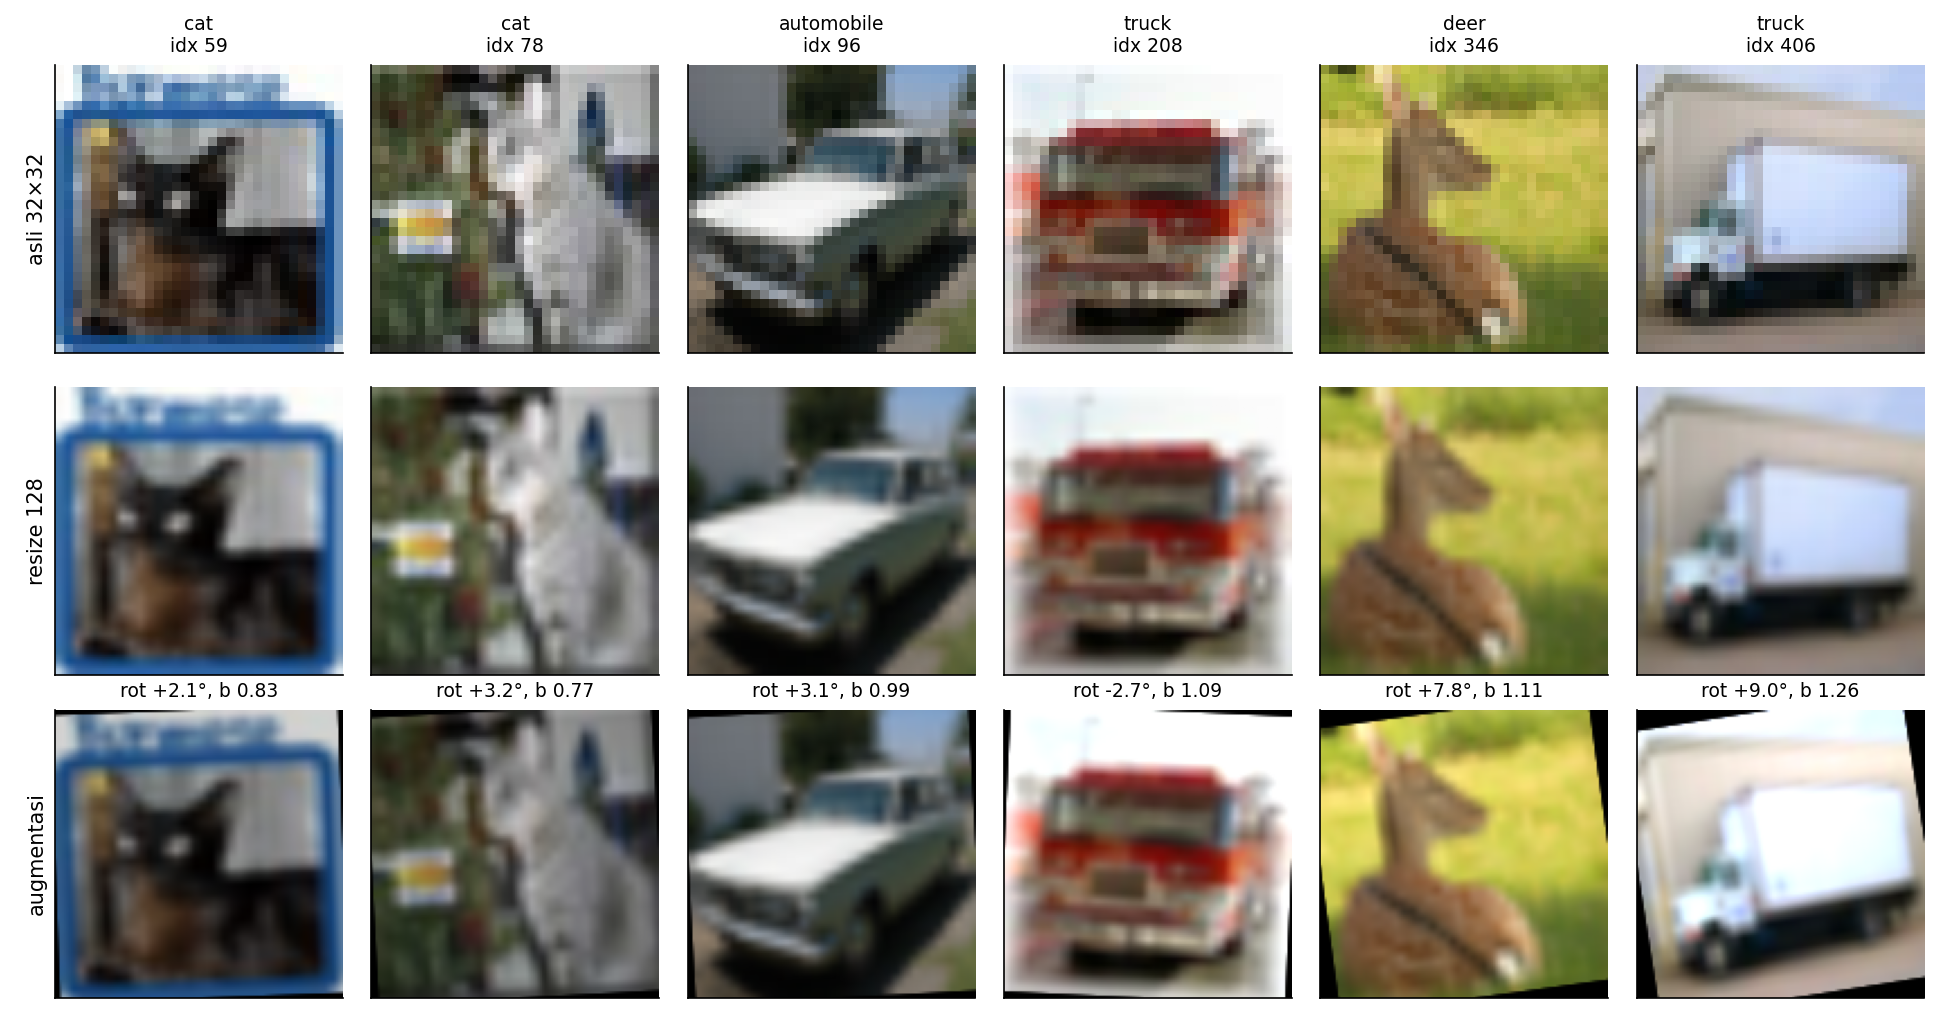
\includegraphics[width=\columnwidth]{preprocessing_augmentasi.png}
\caption{Enam citra \emph{train} pertama: citra asli 32$\times$32, hasil \emph{resize} 128$\times$128, dan versi augmentasinya beserta sudut rotasi dan faktor \emph{brightness}.}
\label{fig:aug}
\end{figure}

\subsection{\emph{Training Linear Head}}

\emph{Head} dilatih dengan \emph{cross-entropy}, \emph{optimizer} Adam dengan \emph{learning rate} 0,001 dan \emph{weight decay} 0, \emph{batch size} 64, selama 30 \emph{epoch}, tanpa \emph{scheduler} maupun \emph{early stopping}. E1 dan E3 dilatih dengan 250 dan 1000 citra bersih, sedangkan E2 dan E4 memakai data yang sama ditambah augmentasi. Pada E2 dan E4, satu \emph{batch} berisi pasangan citra bersih $x$ dan versi augmentasinya $\tilde{x}$, dengan \emph{loss}
\begin{equation}
\mathcal{L} = 0{,}5\,\mathrm{CE}\big(z(x), y\big) + 0{,}5\,\mathrm{CE}\big(z(\tilde{x}), y\big)
\end{equation}
dan satu langkah \emph{optimizer} per \emph{batch}.

Supaya perbandingan adil, untuk setiap \emph{seed} (11, 22, 33) dibuat satu \emph{head} awal yang disimpan, lalu dimuat ulang oleh keempat eksperimen. \emph{Seed} di-\emph{reset} sebelum \emph{head} dan pemuat data dibuat, dan urutan \emph{shuffle} memakai generator terpisah dengan \emph{seed} $s + 1000$, dengan $s$ adalah \emph{training seed}. \emph{Checkpoint} dipilih dari macro-F1 \emph{validation} bersih tertinggi. Kalau ada nilai yang sama, \emph{epoch} yang lebih awal dipilih. Data \emph{test} tidak dipakai selama \emph{training} maupun pemilihan \emph{checkpoint}. Ringkasan konfigurasi ada di Tabel~\ref{tab:config}.

\begin{table}[t]
\caption{Konfigurasi model dan \emph{training}}
\label{tab:config}
\centering
\begin{tabular}{@{}l>{\raggedright\arraybackslash}p{5.3cm}@{}}
\toprule
Parameter & Nilai \\
\midrule
\emph{Backbone} & MobileNetV2, \texttt{IMAGENET1K\_V1}, beku \\
\emph{Input} & 128$\times$128, \emph{bilinear antialias}, normalisasi ImageNet \\
Fitur & 1280 dimensi (\emph{global average pooling}) \\
\emph{Head} & \texttt{Linear(1280, 10)} \\
Augmentasi & rotasi $U(-10^\circ, 10^\circ)$ lalu \emph{brightness} $U(0{,}7;\ 1{,}3)$ \\
\emph{Loss} & \emph{cross-entropy}; E2/E4 memakai persamaan (1) \\
\emph{Optimizer} & Adam, \emph{learning rate} 0,001, \emph{weight decay} 0 \\
\emph{Batch} / \emph{epoch} & 64 / 30, tanpa \emph{scheduler} dan \emph{early stopping} \\
\emph{Checkpoint} & macro-F1 \emph{validation} bersih tertinggi \\
\emph{Seed} & \emph{split} 2026/3026; \emph{training} 11, 22, 33; \emph{shuffle seed} + 1000 \\
\bottomrule
\end{tabular}
\end{table}

\subsection{Evaluasi}

Setiap \emph{checkpoint} dievaluasi pada tujuh kondisi \emph{test}, yaitu bersih, gelap ringan dan sedang (faktor \emph{brightness} 0,8 dan 0,6), \emph{blur} Gaussian ringan dan sedang (\emph{kernel} 5, $\sigma$ 0,6 dan 1,2), serta rotasi ringan dan sedang (+10° dan +20°, \emph{bilinear}, isi 0). Setiap gangguan diterapkan sendiri pada citra bersih yang sudah di-\emph{resize}, tanpa ditumpuk (Gambar~\ref{fig:cond}).

Metrik yang dihitung adalah \emph{accuracy}, \emph{macro-precision}, \emph{macro-recall}, dan macro-F1 atas sepuluh kelas memakai scikit-learn. Kelas yang tidak pernah diprediksi diberi nilai \emph{precision} 0. Karena \emph{test} seimbang (100 citra per kelas), \emph{accuracy} selalu sama dengan \emph{macro-recall}. Hasil dilaporkan per \emph{seed} serta sebagai \emph{mean} $\pm$ \emph{sample standard deviation} dari tiga \emph{seed}. Penurunan akibat gangguan dihitung per \emph{seed} sebagai $\Delta\mathrm{F1} = \mathrm{F1}_{\text{bersih}} - \mathrm{F1}_{\text{terganggu}}$ dan ditulis dalam \emph{percentage points} (pp). Dengan hanya tiga \emph{seed}, \emph{mean} $\pm$ std dipakai untuk menggambarkan sebaran, bukan sebagai uji signifikansi.

\begin{figure}[t]
\centering
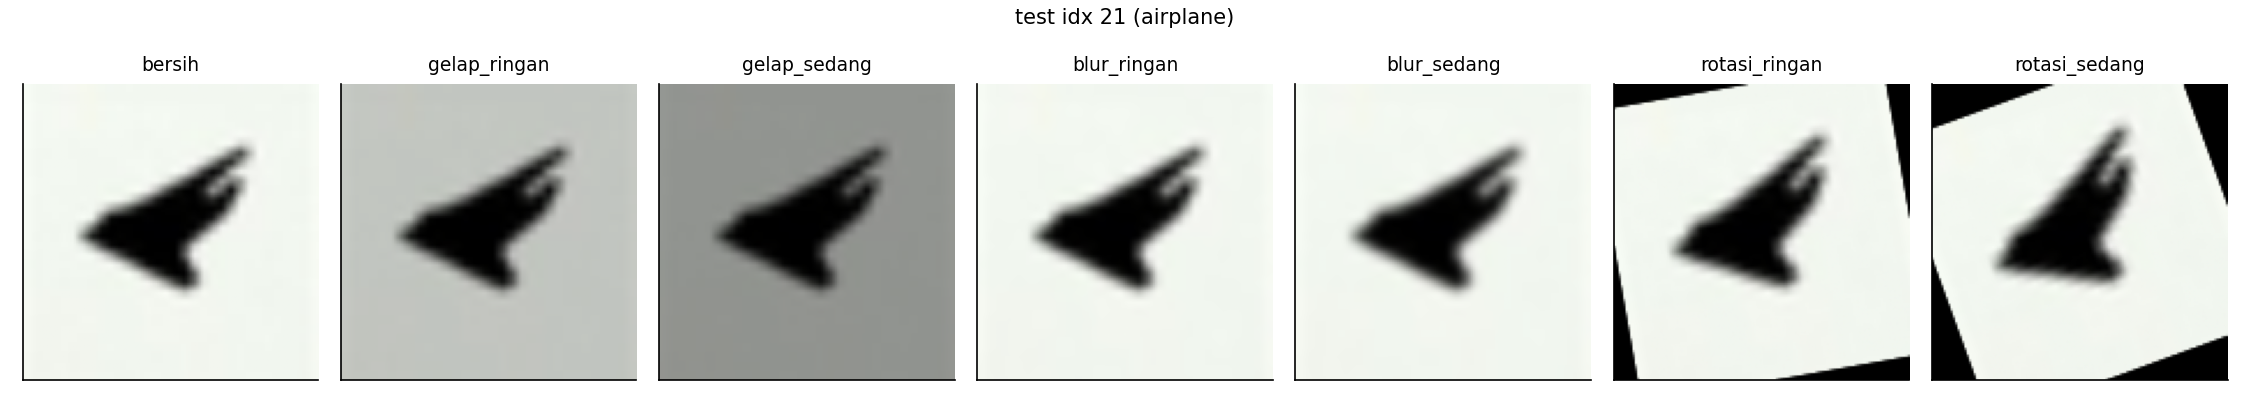
\includegraphics[width=\columnwidth]{kondisi_test.png}
\caption{Tujuh kondisi \emph{test} pada citra \emph{test} pertama.}
\label{fig:cond}
\end{figure}

\subsection{Lingkungan dan \emph{Reproducibility}}\label{sec:repro}

Semua \emph{run} dijalankan di Google Colab versi gratis dengan \emph{runtime} CPU (Intel Xeon 2,20 GHz, 2 \emph{core}) menggunakan PyTorch 2.14.1 dan torchvision 0.29.1. Ekstraksi fitur untuk 9500 citra memakan waktu 190 detik, dan \emph{training} 12 \emph{head} total sekitar 8 detik. \emph{Split}, \emph{checkpoint}, prediksi, dan metrik disimpan bersama \emph{checksum} SHA-256. \emph{Notebook} juga punya mode verifikasi yang memuat artefak tersebut, menghitung ulang prediksi dan metrik tanpa \emph{training}, lalu mencocokkannya dengan \emph{file} yang tersimpan. Untuk menguji konsistensi antar-mesin, \emph{notebook} yang sama juga dijalankan di laptop dengan arsitektur CPU dan versi \emph{library} yang berbeda.

\section{Hasil}\label{sec:results}

Mode verifikasi di Colab menghasilkan prediksi dan metrik yang sama dengan \emph{file} tersimpan, dan semua \emph{checksum} cocok. Dibandingkan dengan \emph{run} di laptop, metrik dan ke-84.000 prediksi kelas sama persis, sedangkan probabilitasnya hanya berbeda di digit keenam (paling jauh 0,000015).

\subsection{\emph{Test} Bersih}\label{sec:res-clean}

Tabel~\ref{tab:clean} menunjukkan hasil pada \emph{test} bersih. E4 memperoleh macro-F1 tertinggi, diikuti E3, E1, dan E2. Selisih akibat jumlah data (4,02 dan 6,78 pp) jauh lebih besar daripada selisih akibat augmentasi (paling jauh 2,09 pp). \emph{Standard deviation} antar-\emph{seed} paling besar 0,24 pp, dan nilai per \emph{seed} pada Tabel~\ref{tab:seed} menunjukkan rentang terlebar 0,47 pp pada E2. Pada \emph{validation}, urutan E3 dan E4 justru terbalik. Macro-F1 \emph{validation} terbaik E3 berkisar 80,59--81,39\%, sedangkan E4 berkisar 79,73--80,42\%.

\begin{table}[t]
\caption{Hasil \emph{test} bersih E1--E4 (\%, \emph{mean} $\pm$ std, 3 \emph{seed})}
\label{tab:clean}
\centering
\setlength{\tabcolsep}{3pt}
\begin{tabular}{@{}lcccc@{}}
\toprule
 & \emph{Accuracy} & Macro-P & Macro-R & Macro-F1 \\
\midrule
\tabinput{tables/hasil_bersih.tex}
\bottomrule
\end{tabular}
\end{table}

\begin{table}[t]
\caption{Macro-F1 \emph{test} bersih per \emph{seed} (\%)}
\label{tab:seed}
\centering
\begin{tabular}{@{}lccc@{}}
\toprule
 & \emph{Seed} 11 & \emph{Seed} 22 & \emph{Seed} 33 \\
\midrule
\tabinput{tables/f1_per_seed.tex}
\bottomrule
\end{tabular}
\end{table}

Kurva \emph{training} pada Gambar~\ref{fig:curve} memperlihatkan bahwa macro-F1 \emph{validation} E3 dan E4 sudah mendatar setelah sekitar 5 \emph{epoch}, sedangkan E1 dan E2 sedikit lebih lambat. Setelah itu nilainya hanya naik turun sedikit, sehingga \emph{best epoch} tersebar antara \emph{epoch} 8 dan 28. \emph{Training loss} E2 dan E4 lebih tinggi daripada E1 dan E3.

\begin{figure}[t]
\centering
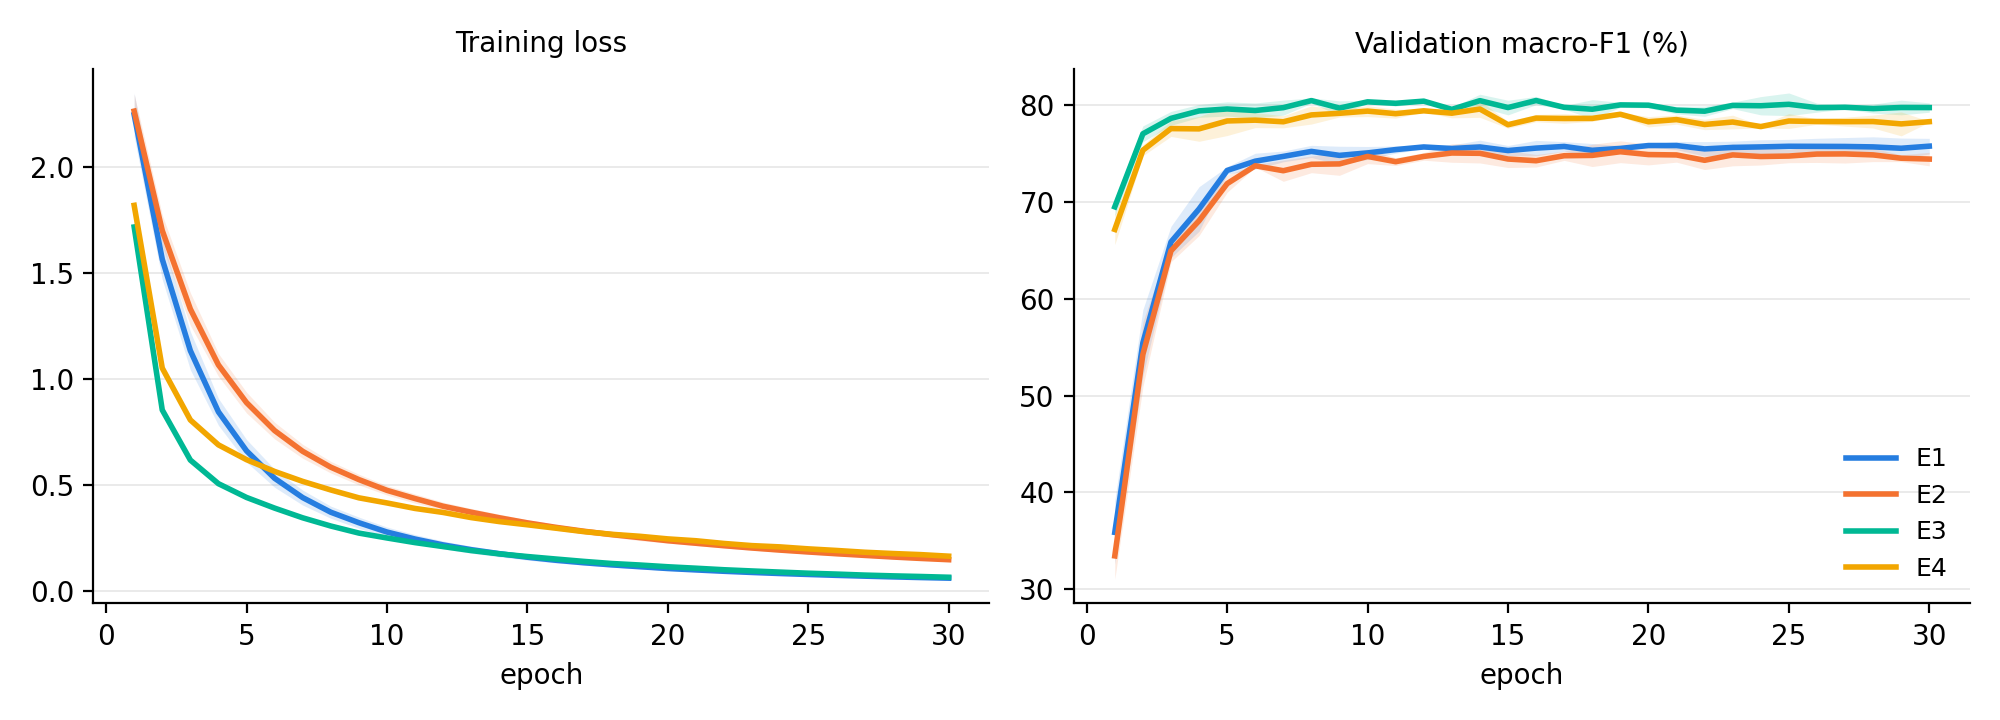
\includegraphics[width=\columnwidth]{kurva_training.png}
\caption{\emph{Training loss} dan macro-F1 \emph{validation} per \emph{epoch}. Garis adalah rata-rata tiga \emph{seed}, area tipis menunjukkan $\pm$1 std.}
\label{fig:curve}
\end{figure}

\subsection{Tujuh Kondisi \emph{Test}}\label{sec:res-cond}

Tabel~\ref{tab:cond} dan Gambar~\ref{fig:delta} merangkum kinerja pada semua kondisi. Gangguan gelap dan \emph{blur} hanya menurunkan macro-F1 sedikit, paling besar 4,62 pp (E4, gelap sedang). Rotasi jauh lebih merusak. Tanpa augmentasi, macro-F1 pada rotasi 20° turun ke 27,42\% (E1) dan 23,61\% (E3), sedangkan dengan augmentasi E2 dan E4 masih mencapai 48,43\% dan 54,73\%.

\begin{table*}[t]
\caption{Macro-F1 pada tujuh kondisi \emph{test} (\%, \emph{mean} $\pm$ std, 3 \emph{seed}). R = ringan, S = sedang.}
\label{tab:cond}
\centering
\begin{tabular}{@{}lccccccc@{}}
\toprule
 & Bersih & Gelap R & Gelap S & \emph{Blur} R & \emph{Blur} S & Rotasi R & Rotasi S \\
\midrule
\tabinput{tables/f1_kondisi.tex}
\bottomrule
\end{tabular}
\end{table*}

\begin{figure}[t]
\centering
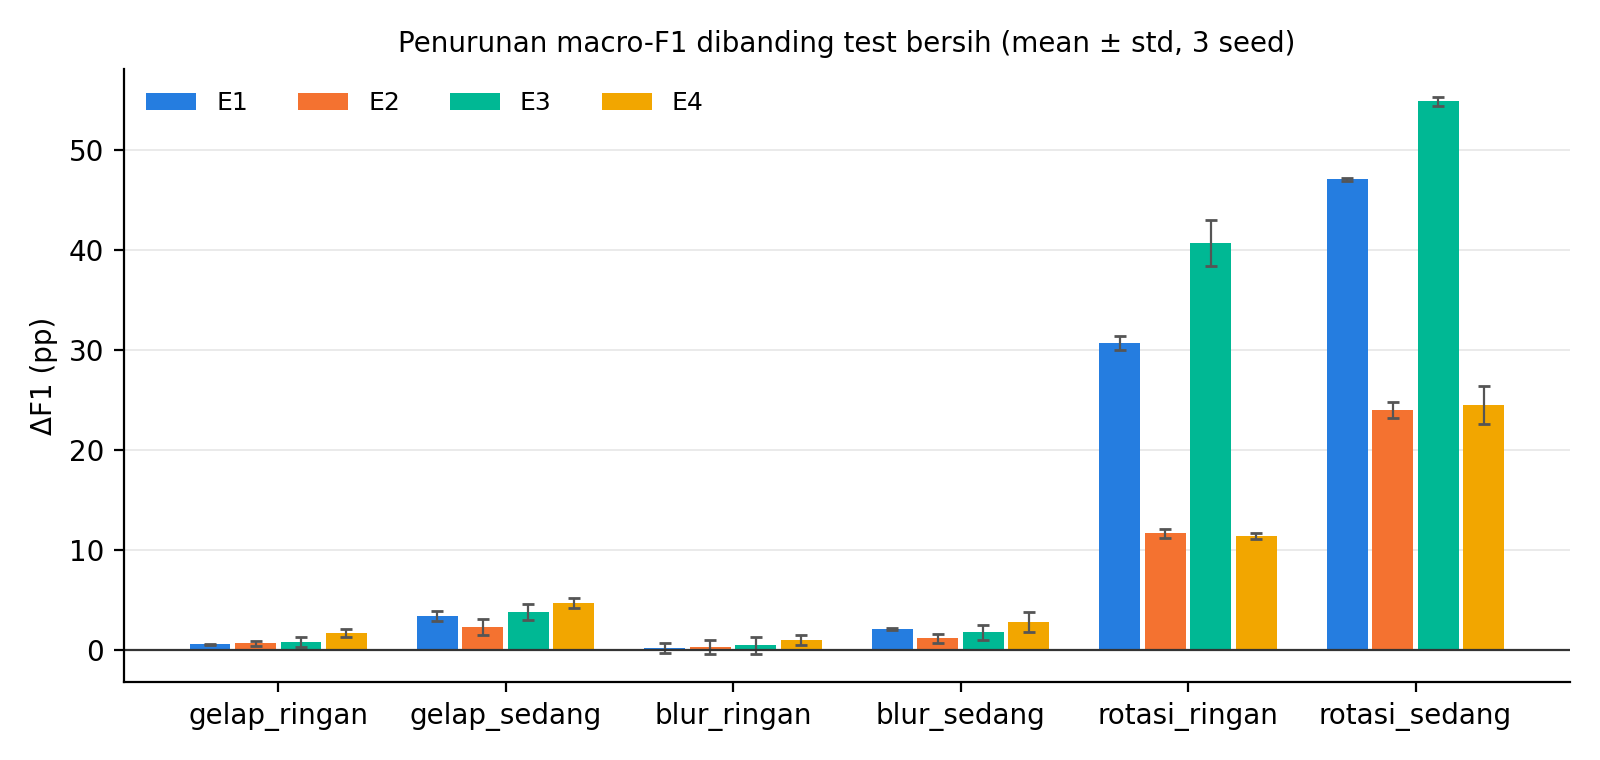
\includegraphics[width=\columnwidth]{delta_f1.png}
\caption{$\Delta$F1 terhadap \emph{test} bersih untuk enam gangguan (\emph{mean} $\pm$ std, 3 \emph{seed}). Nilai positif berarti macro-F1 turun.}
\label{fig:delta}
\end{figure}

\subsection{Konsistensi Antar-\emph{Seed}}\label{sec:res-cons}

Tabel~\ref{tab:cons} memuat selisih macro-F1 antar-eksperimen yang dihitung per \emph{seed} lalu dirata-rata. Tanda $\dagger$ menandai selisih yang arahnya tidak sama di ketiga \emph{seed}. Dari 28 perbandingan, 24 punya arah yang sama di ketiga \emph{seed}. Empat yang tidak konsisten semuanya berasal dari E4 $-$ E3 pada gangguan gelap dan \emph{blur}, dengan rata-rata selisih paling besar 0,34 pp.

\begin{table*}[t]
\caption{Rata-rata selisih macro-F1 antar-eksperimen (pp), dihitung per \emph{seed}. $\dagger$: arah selisih tidak sama di ketiga \emph{seed}.}
\label{tab:cons}
\centering
\begin{tabular}{@{}lccccccc@{}}
\toprule
Perbandingan & Bersih & Gelap R & Gelap S & \emph{Blur} R & \emph{Blur} S & Rotasi R & Rotasi S \\
\midrule
\tabinput{tables/konsistensi.tex}
\bottomrule
\end{tabular}
\end{table*}

\subsection{Kesalahan Klasifikasi}

Gambar~\ref{fig:cm} menunjukkan \emph{confusion matrix} E3 dan E4 pada \emph{test} bersih untuk \emph{seed} 11. Pasangan yang paling sering tertukar di keempat eksperimen adalah cat dan dog. Jika dijumlahkan atas tiga \emph{seed}, jumlahnya 85 kesalahan pada E1, 80 pada E2, 102 pada E3, dan 103 pada E4 (dua arah digabung). Pasangan berikutnya adalah deer--horse, airplane--ship, dan automobile--truck. Beberapa kesalahan tidak simetris. Pada E4, automobile diprediksi truck 36 kali, tetapi truck diprediksi automobile hanya 7 kali.

\begin{figure*}[t]
\centering
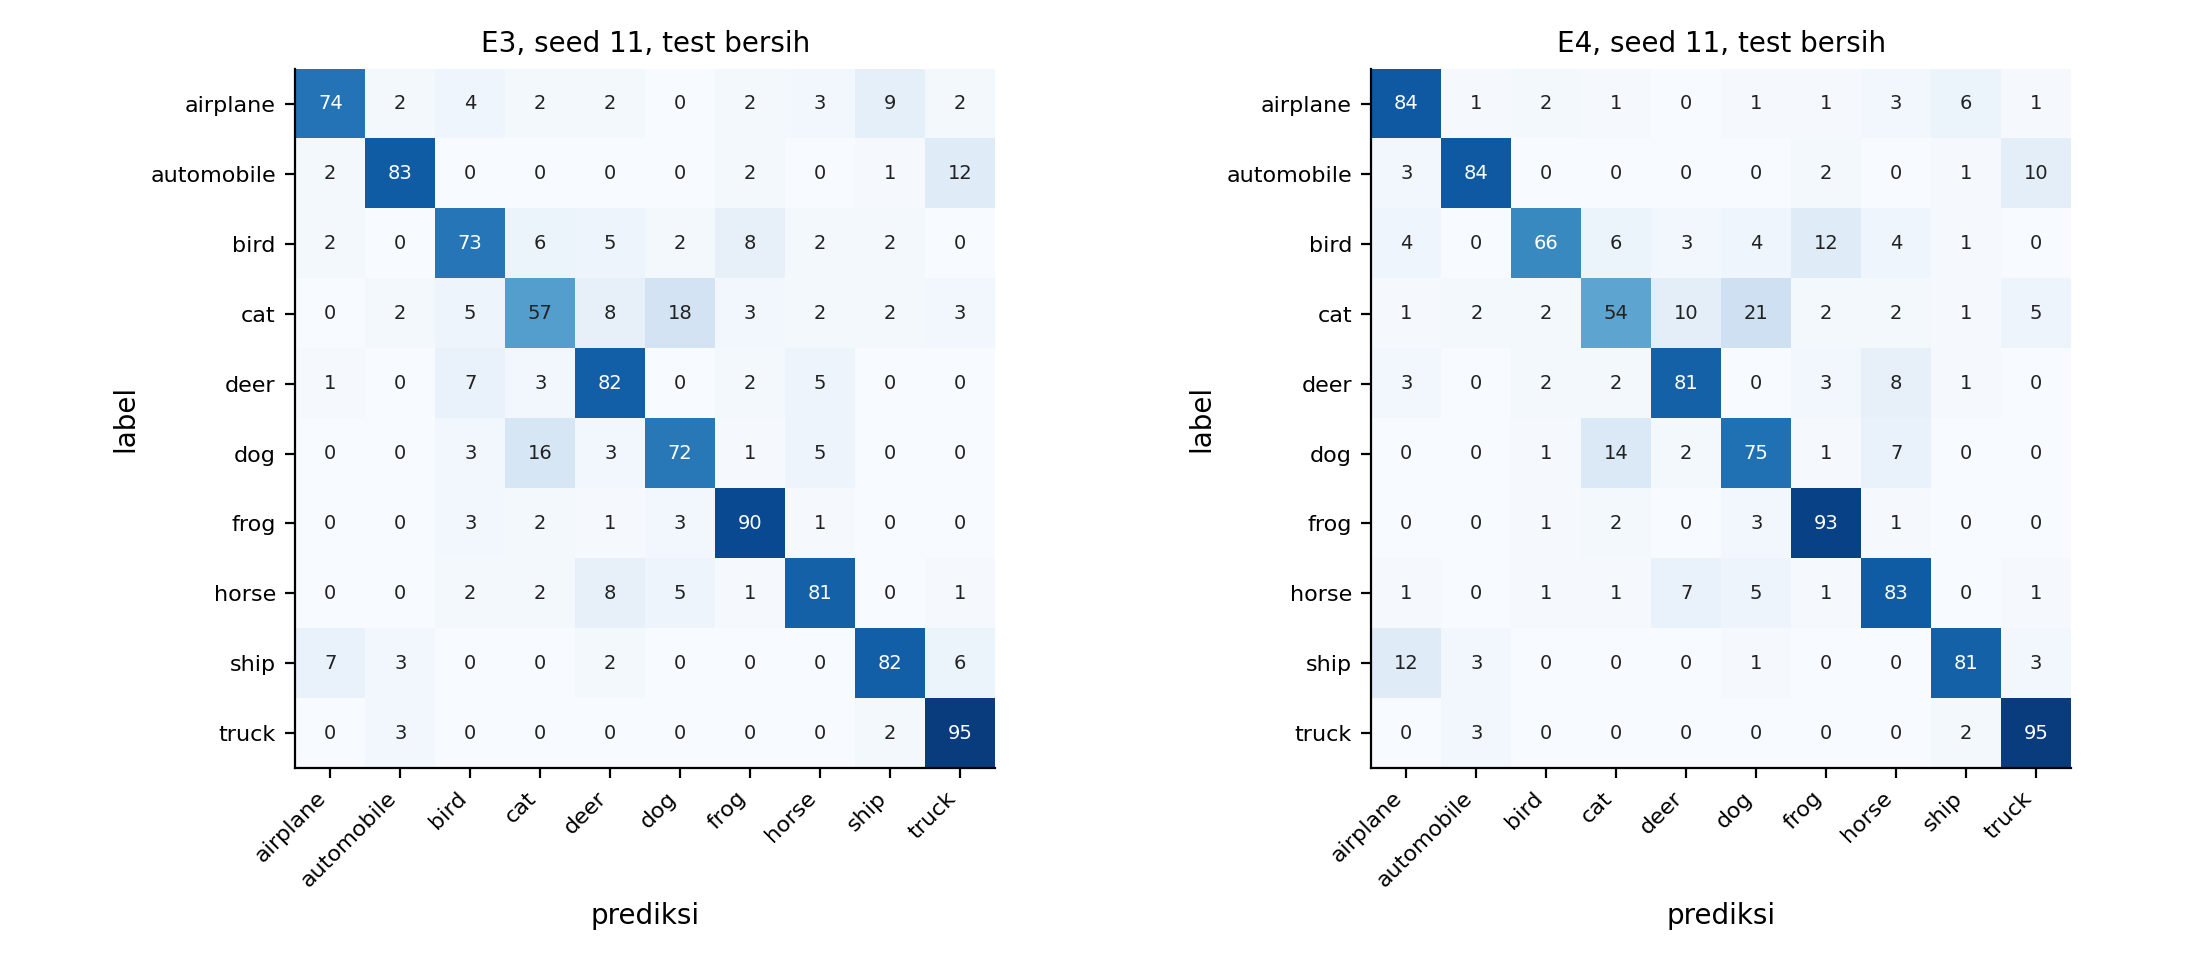
\includegraphics[width=0.82\textwidth]{confusion_matrix_E3_E4.png}
\caption{\emph{Confusion matrix} E3 dan E4 pada \emph{test} bersih, \emph{seed} 11.}
\label{fig:cm}
\end{figure*}

Gambar~\ref{fig:samples} memperlihatkan dua belas sampel \emph{test} pertama pada kondisi bersih dan tiga gangguan tingkat sedang, dengan prediksi E4 \emph{seed} 11. Gambar~\ref{fig:err} menampilkan enam kesalahan pertama E4 \emph{seed} 11 pada \emph{test} bersih. Tiga di antaranya adalah bird yang diprediksi frog. Kesalahan dengan \emph{confidence} tertinggi (0,90) adalah burung di latar gelap.

\begin{figure*}[t]
\centering
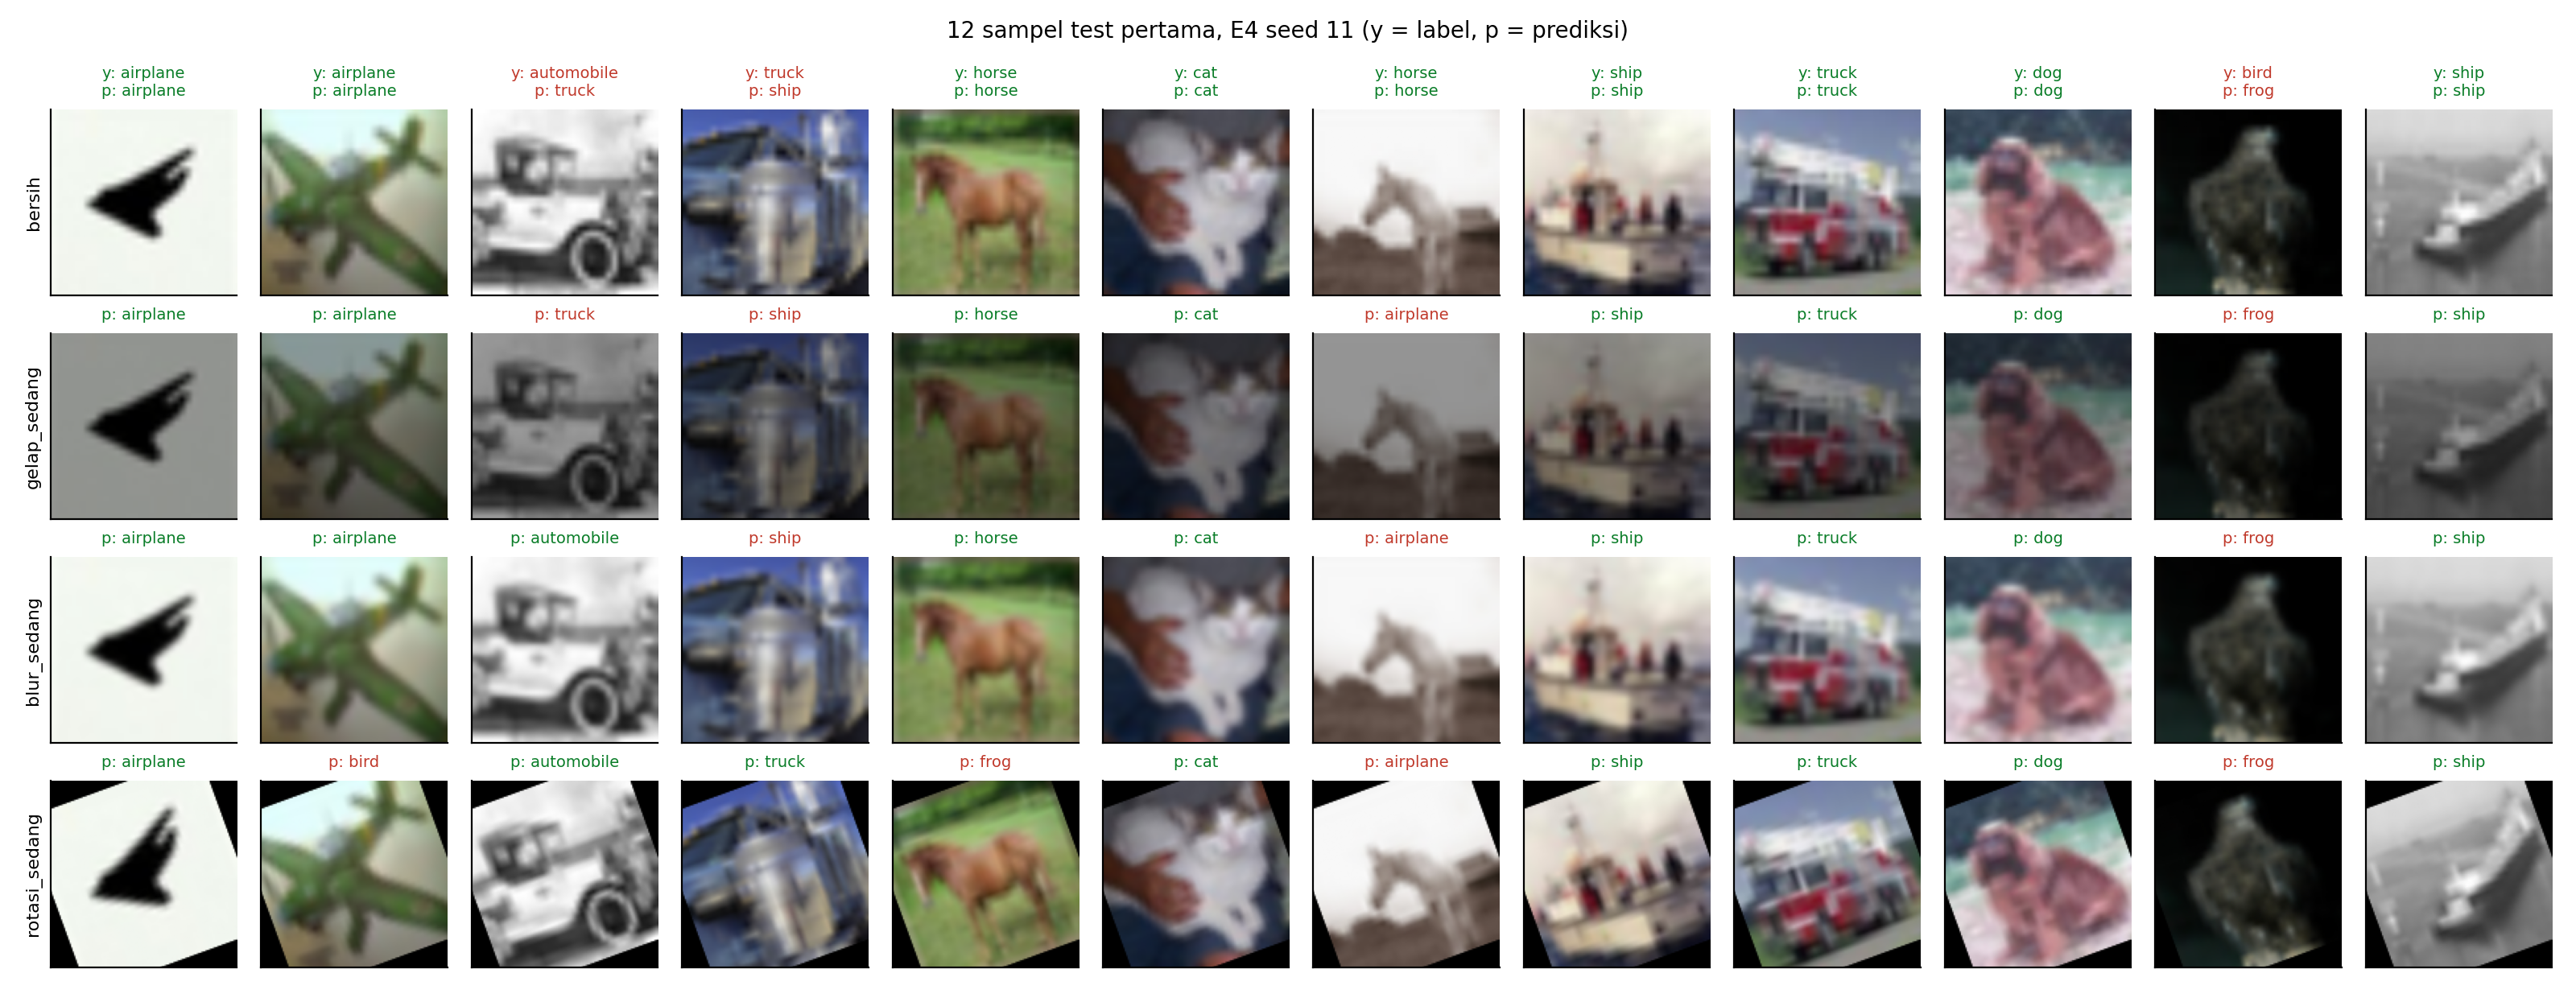
\includegraphics[width=\textwidth]{sampel_test_pertama.png}
\caption{Dua belas sampel \emph{test} pertama pada kondisi bersih, gelap sedang, \emph{blur} sedang, dan rotasi sedang dengan prediksi E4 \emph{seed} 11. Hijau berarti benar, merah berarti salah.}
\label{fig:samples}
\end{figure*}

\begin{figure*}[t]
\centering
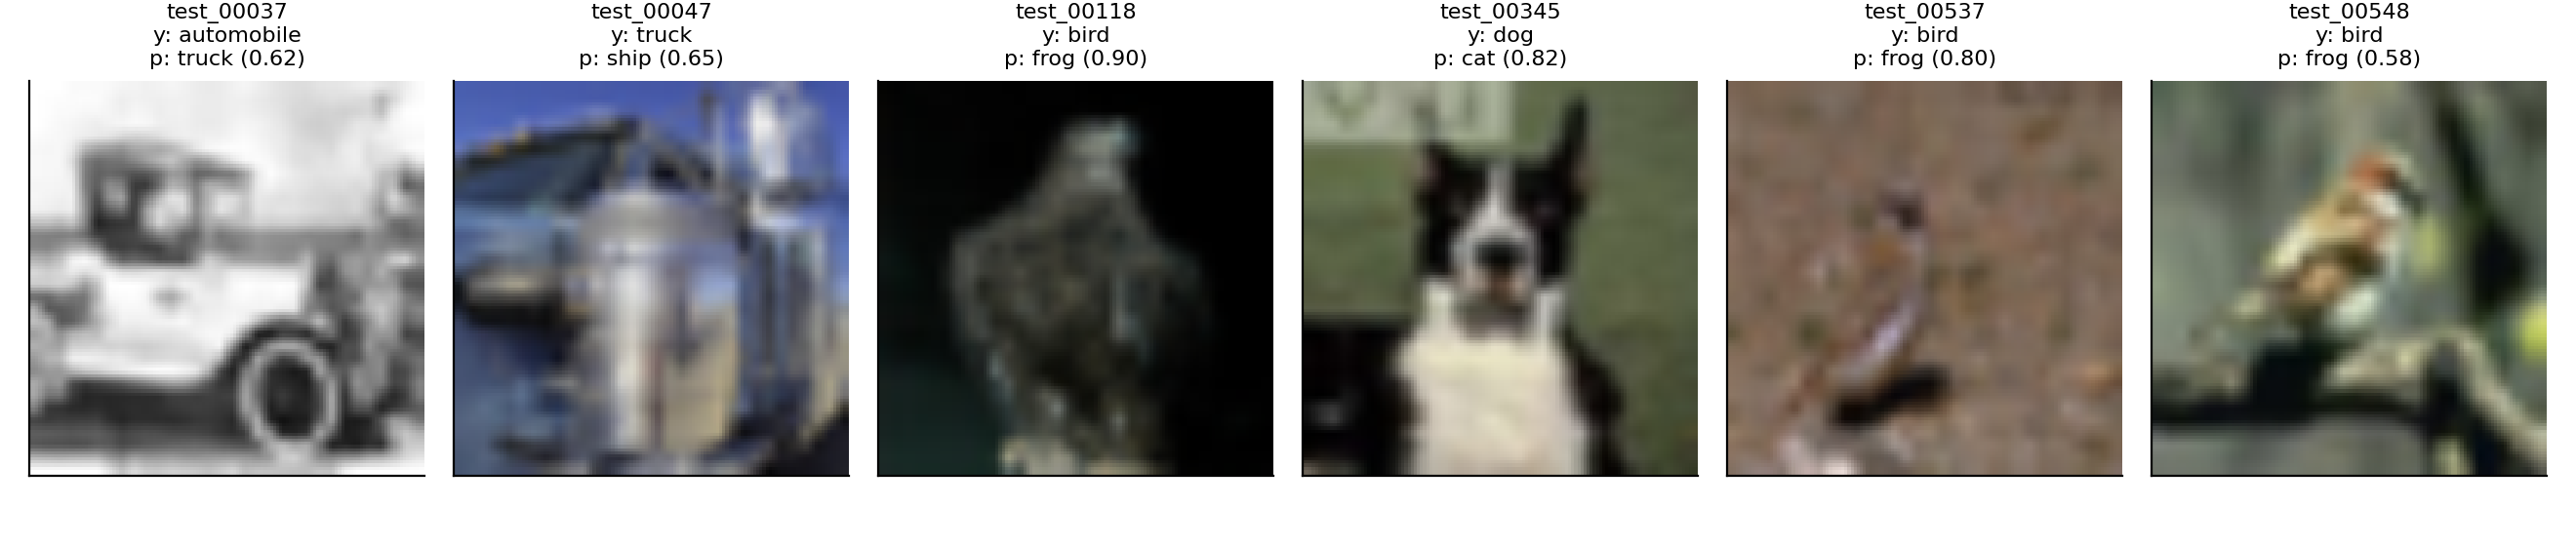
\includegraphics[width=0.85\textwidth]{contoh_kesalahan.png}
\caption{Enam kesalahan prediksi pertama E4 \emph{seed} 11 pada \emph{test} bersih beserta \emph{confidence} prediksinya.}
\label{fig:err}
\end{figure*}

\section{Pembahasan}\label{sec:discussion}

\subsection{Dampak Pengurangan Data}

Mengurangi data dari 1000 menjadi 250 citra menurunkan macro-F1 \emph{test} bersih, dengan arah yang sama di ketiga \emph{seed}. Penurunan ini relatif kecil mengingat datanya tinggal seperempat. Fitur ImageNet sudah cukup memisahkan kelas-kelas CIFAR-10, sehingga \emph{linear head} dengan 25 contoh per kelas pun mencapai macro-F1 sekitar 74,5\%. Hal ini sejalan dengan temuan Kornblith dkk.\ \cite{kornblith2019better} tentang kuatnya fitur tetap.

Satu pengecualian muncul pada rotasi. Tanpa augmentasi, E3 justru lebih buruk daripada E1 pada kedua tingkat rotasi (Tabel~\ref{tab:cons}). Salah satu kemungkinan penjelasannya, dengan lebih banyak contoh tegak, \emph{head} E3 menyesuaikan diri lebih ketat pada distribusi fitur citra tegak, sehingga lebih mudah salah ketika distribusinya bergeser. Eksperimen ini belum cukup untuk memastikan hal tersebut.

\subsection{Augmentasi pada \emph{Test} Bersih}

Efek augmentasi pada \emph{test} bersih bergantung pada jumlah data. Augmentasi menurunkan macro-F1 pada 250 citra, tetapi sedikit menaikkannya pada 1000 citra, dan kedua arah ini konsisten di ketiga \emph{seed}. Penjelasan yang paling mungkin adalah keterbatasan kapasitas. Dengan \emph{loss} 50:50, \emph{head} linear harus memisahkan kelas sekaligus pada fitur bersih dan fitur citra yang dirotasi. Rotasi menggeser fitur cukup jauh, dan dengan hanya 25 contoh per kelas kompromi ini mengorbankan kinerja pada citra bersih. \emph{Training loss} E2 dan E4 yang lebih tinggi (Gambar~\ref{fig:curve}) sejalan dengan hal ini. Dengan 1000 citra, kedua distribusi terwakili lebih baik. Meski begitu, kenaikan pada 1000 citra kecil dan tidak terlihat pada \emph{validation}.

\subsection{Gangguan yang Sejenis dengan Augmentasi}

Augmentasi yang dipakai sejenis dengan dua gangguan \emph{test}, yaitu rotasi dan gelap. Untuk rotasi, manfaatnya besar dan konsisten. $\Delta$F1 pada rotasi 20° berkurang kira-kira setengahnya, baik pada 250 maupun 1000 citra (Gambar~\ref{fig:delta}). Manfaat ini muncul walaupun rotasi 20° berada di luar rentang augmentasi ($\pm$10°). Walau begitu, rotasi tetap menjadi gangguan paling berat. Temuan ini tidak bertentangan dengan Engstrom dkk.\ \cite{engstrom2019spatial} yang melaporkan augmentasi hanya sedikit membantu, karena di sana sudut rotasi dipilih yang paling merugikan model, sedangkan di sini sudutnya tetap.

Untuk gangguan gelap, augmentasi \emph{brightness} tidak membantu. Pada 1000 citra, selisih E4 $-$ E3 kecil dan arahnya berbeda antar-\emph{seed}, bahkan $\Delta$F1 E4 sedikit lebih besar daripada E3. Kemungkinan penyebabnya, gangguan gelap memang hanya sedikit menurunkan kinerja model tanpa augmentasi, sehingga ruang perbaikannya kecil. Dodge dan Karam \cite{dodge2016quality} juga melaporkan bahwa perubahan kontras berdampak kecil pada CNN. Selain itu, setiap citra augmentasi selalu dirotasi sekaligus diubah \emph{brightness}-nya, sehingga efek kedua augmentasi tidak bisa dipisahkan.

\subsection{Perpindahan Manfaat ke Gangguan Lain}

Manfaat augmentasi tidak berpindah ke \emph{blur}. Pada 1000 citra, selisih E4 $-$ E3 pada kedua tingkat \emph{blur} kurang dari 0,4 pp dengan arah yang tidak konsisten. Pada 250 citra, E2 tetap lebih buruk daripada E1, dengan selisih yang mirip dengan penurunan pada \emph{test} bersih. \emph{Blur} sendiri hanya berdampak kecil di eksperimen ini. Citra 32$\times$32 yang diperbesar empat kali dengan interpolasi \emph{bilinear} sudah halus, dan $\sigma = 1{,}2$ pada resolusi 128 setara dengan sekitar 0,3 piksel pada citra asli.

\subsection{Kelas yang Paling Sering Tertukar}

Pasangan yang paling sering tertukar memang mirip secara visual pada resolusi 32$\times$32. Pada airplane--ship, latar langit dan laut yang sama-sama biru kemungkinan ikut berperan. Tambahan data dari E1 ke E3 tidak mengurangi kebingungan cat--dog. Jumlahnya justru naik dari 85 menjadi 102, sementara pasangan lain seperti airplane--ship turun dari 72 menjadi 46. Artinya, fitur MobileNetV2 beku pada resolusi ini tampaknya kurang mampu membedakan cat dan dog, sehingga menambah data untuk \emph{head} linear saja tidak cukup.

\subsection{Konsistensi Antar-\emph{Seed}}

Pola pada Tabel~\ref{tab:cons} menunjukkan bahwa efek jumlah data dan efek augmentasi terhadap rotasi cukup stabil. Sebaliknya, efek augmentasi pada gelap dan \emph{blur} untuk 1000 citra terlalu kecil untuk dibedakan dari variasi antar-\emph{seed}. Perlu diingat bahwa ketiga \emph{seed} hanya mengubah inisialisasi \emph{head} dan urutan \emph{shuffle}. \emph{Split} dan fitur sama untuk semua \emph{seed}, jadi \emph{standard deviation} di sini belum mencakup variasi akibat pemilihan sampel data, yang menurut Bouthillier dkk.\ \cite{bouthillier2021variance} juga berpengaruh nyata.

\section{Keterbatasan}

\emph{Backbone} yang beku berarti model hanya bisa belajar batas keputusan linear di atas fitur yang sudah tetap. Augmentasi tidak dapat membuat fitur itu sendiri tahan rotasi. Augmentasi hanya mengajari \emph{head} untuk mengenali kelas dari fitur citra yang dirotasi. MobileNetV2 juga dilatih pada citra ImageNet beresolusi lebih tinggi, sedangkan \emph{input} di sini adalah citra 32$\times$32 yang diperbesar ke 128$\times$128, sehingga ada perbedaan domain yang tidak bisa dikoreksi tanpa \emph{fine-tuning}. Karena itu, temuan ini belum tentu berlaku ketika \emph{backbone} ikut dilatih.

Ukuran \emph{subset} kecil. \emph{Test} hanya berisi 100 citra per kelas, sehingga satu citra setara 1 pp \emph{recall} kelas tersebut dan 0,1 pp \emph{accuracy}. \emph{Validation} hanya 50 citra per kelas, dan urutan E3 dan E4 yang terbalik antara \emph{validation} dan \emph{test} menunjukkan bahwa \emph{validation} sekecil ini belum cukup untuk membedakan selisih di bawah 1 pp. Hanya ada satu \emph{split} dan tiga \emph{seed}, sehingga \emph{standard deviation} yang dilaporkan kemungkinan meremehkan variasi sebenarnya. Mengulang eksperimen dengan beberapa \emph{split} berbeda akan memberi gambaran variasi yang lebih lengkap. Selain itu, hanya satu \emph{backbone} dan satu \emph{dataset} yang diuji, sehingga generalisasi hasilnya masih terbatas.

Gangguannya sintetis dan sederhana. Setiap jenis gangguan hanya punya dua tingkat dengan satu parameter tetap, rotasi hanya ke satu arah, dan \emph{brightness} hanya digelapkan. Area kosong akibat rotasi diisi hitam, sehingga muncul sudut hitam di tepi citra. Karena citra augmentasi juga punya sudut hitam, sebagian manfaat augmentasi mungkin berasal dari \emph{head} yang belajar mengabaikan artefak itu, bukan dari kemampuan mengenali objek yang miring. Selain itu, rotasi dan \emph{brightness} selalu diterapkan bersama, sehingga efek masing-masing augmentasi tidak bisa dipisahkan. Menguji tiap augmentasi secara terpisah, memakai rotasi dua arah, dan mengganti cara pengisian tepi akan membantu memisahkan kemungkinan-kemungkinan tersebut. Gangguan nyata seperti \emph{noise}, kompresi, oklusi, atau kombinasi beberapa gangguan juga belum diuji.

\section{Kesimpulan}\label{sec:conclusion}

Penelitian ini menunjukkan bahwa dengan MobileNetV2 beku dan \emph{linear head}, jumlah data berpengaruh lebih besar daripada augmentasi terhadap kinerja pada \emph{test} bersih. Menambah data dari 250 ke 1000 citra menaikkan macro-F1 sekitar 4 sampai 7 pp secara konsisten, sedangkan augmentasi rotasi dan \emph{brightness} justru merugikan pada 250 citra dan hanya sedikit membantu pada 1000 citra. Manfaat augmentasi hampir seluruhnya terbatas pada rotasi, dengan penurunan macro-F1 akibat rotasi 20° berkurang kira-kira setengahnya, dan tidak terlihat pada gangguan gelap maupun \emph{blur}. Jadi, augmentasi sebaiknya dipilih sesuai gangguan yang benar-benar diperkirakan muncul, bukan diharapkan memberi ketahanan secara umum. Hasilnya juga dapat dihitung ulang dan konsisten di mesin yang berbeda. Penelitian berikutnya dapat membandingkan hasil ini dengan \emph{fine-tuning} dan menguji tiap augmentasi secara terpisah.

\bibliographystyle{IEEEtran}
\bibliography{references}

\end{document}
